Raspberri Pi is connected to elevator via serial cable.
Elevator movement can be controlled via serial port by sending commands to it in binary form.

% we need a few pics here when we finish the setup
%\begin{figure}
%\center{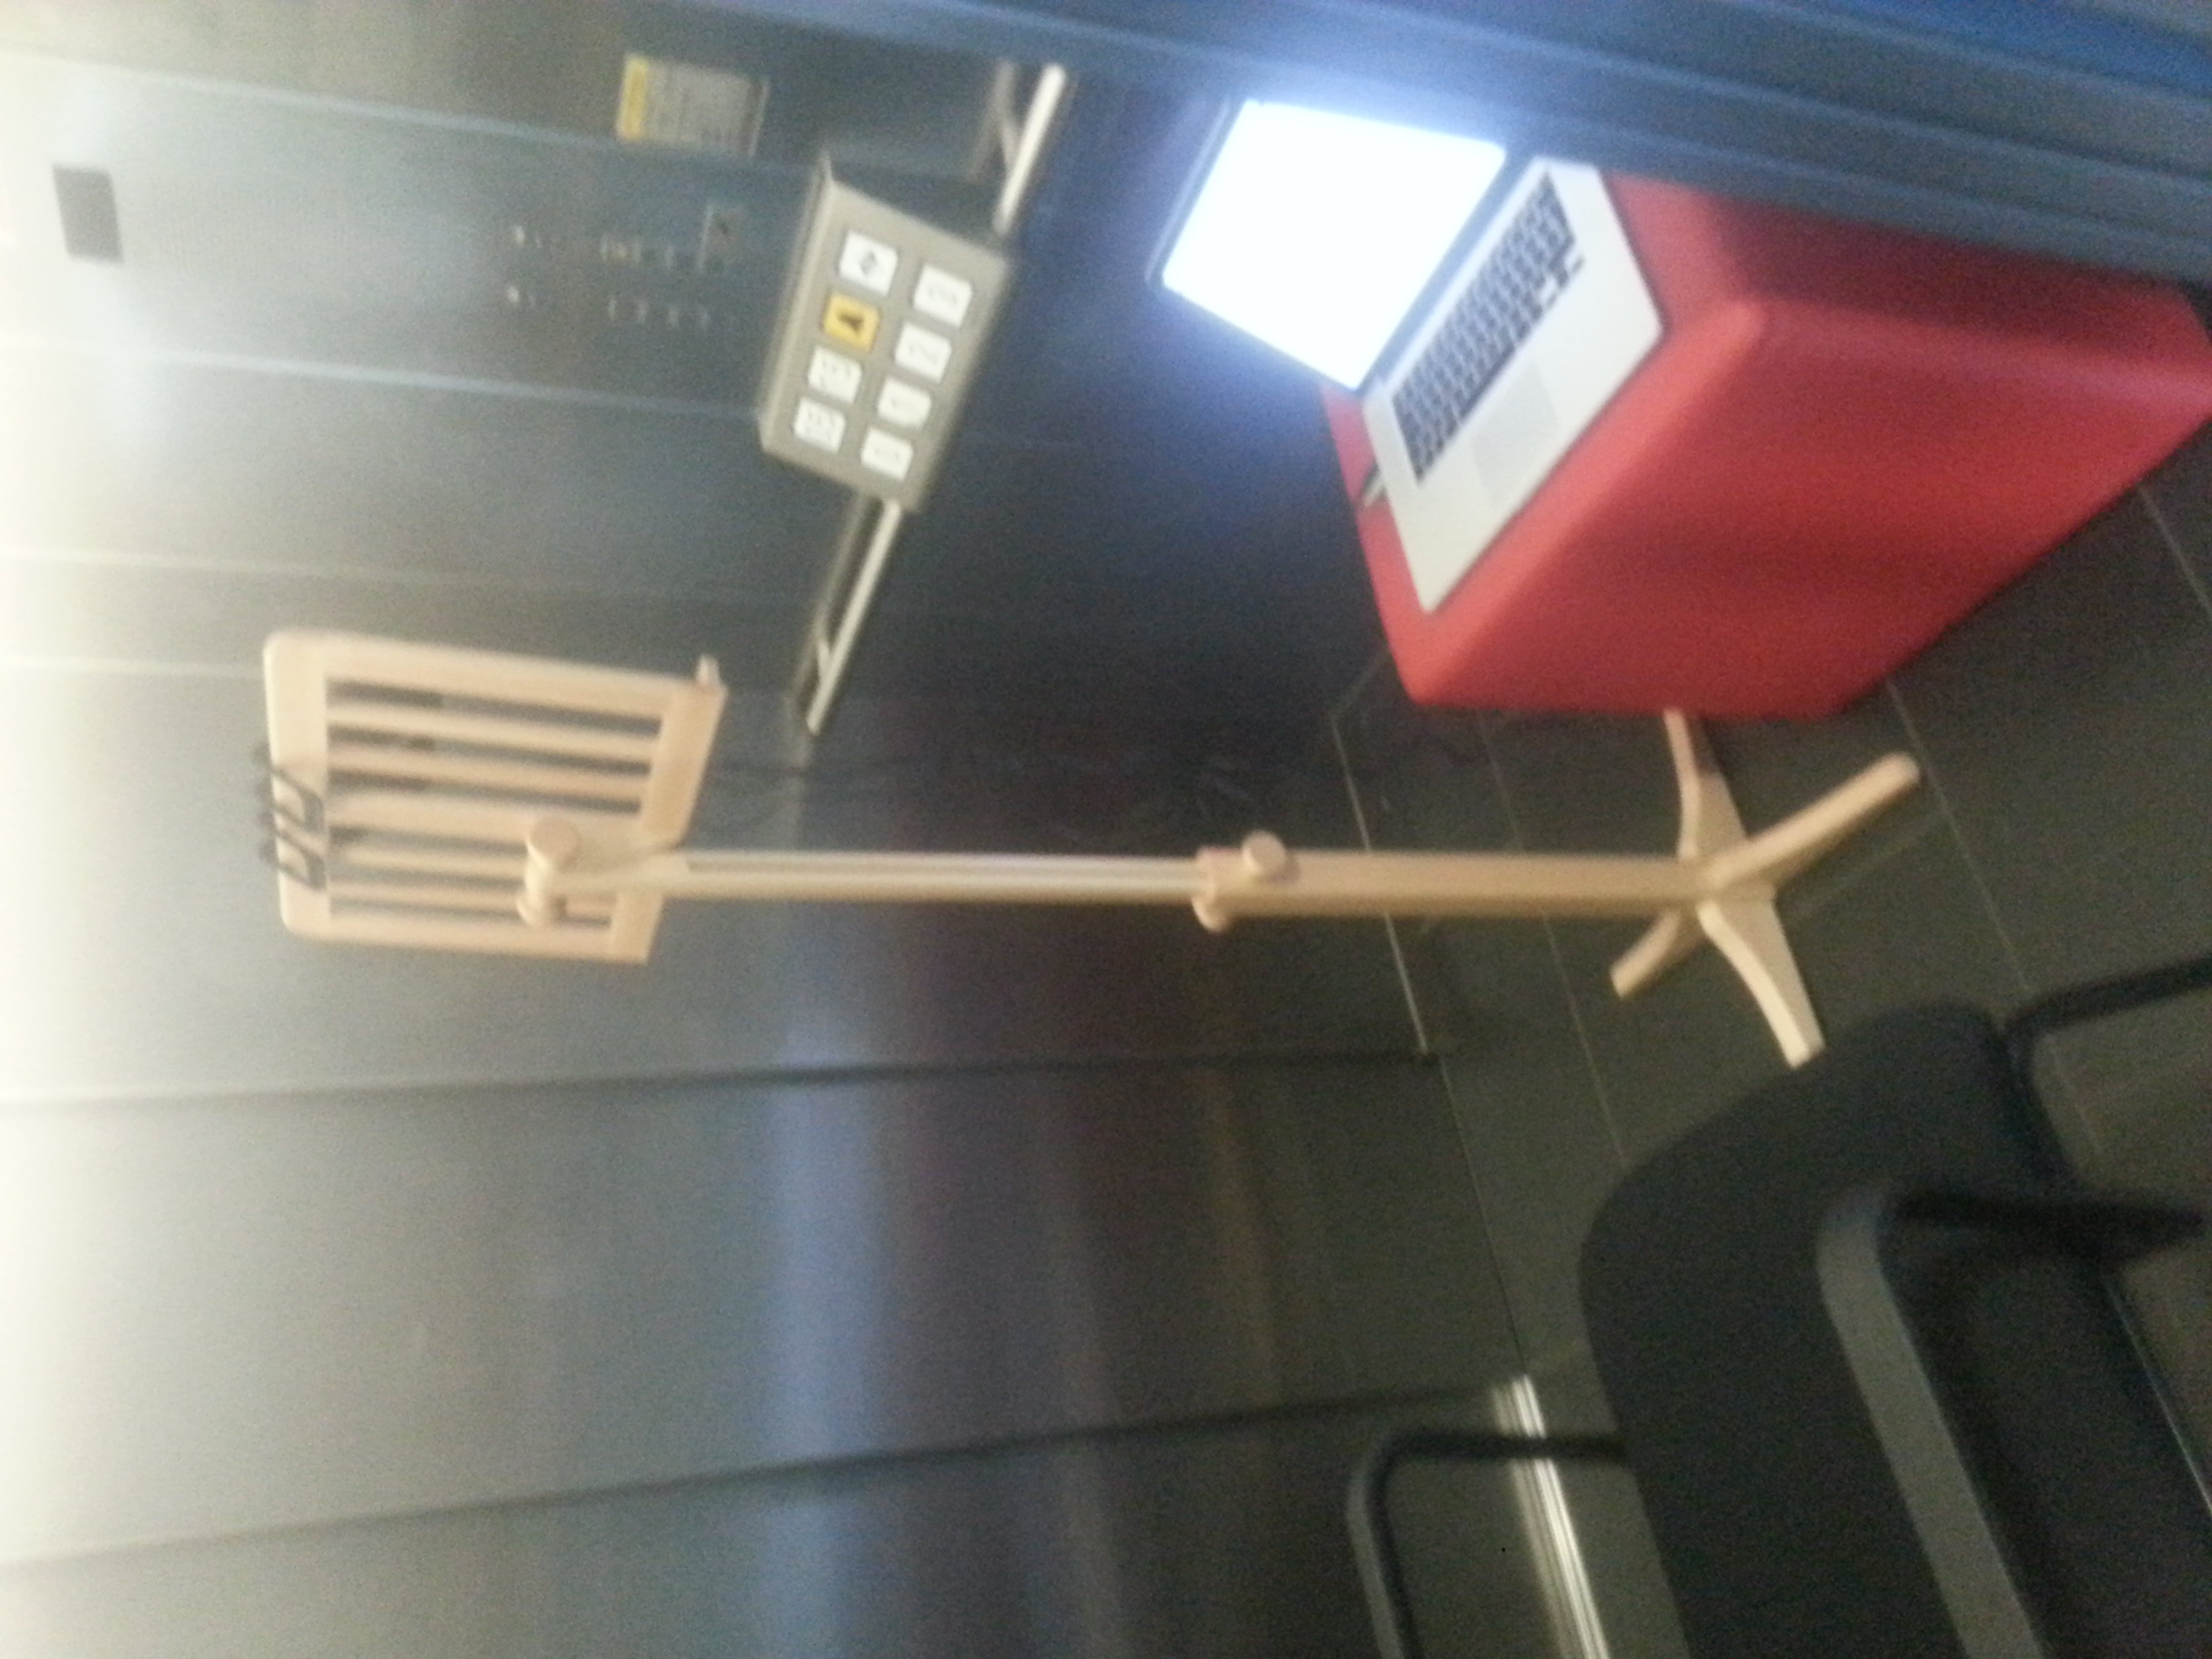
\includegraphics[scale=0.10, angle=-90]{setup_reverberation_rec.jpg}}
%\caption{Recordings setup.}
%\label{fig:recordingsetup}
%\end{figure}


Before implementation we reviewed several java libraries for serial communication: pi4j, javax.comm, RXTX.
It was decided to use RXTX, because pi4j was not stable enough and javax.comm turned out to be buggy without freely available sources.
There are a few classes that handle serial connection and data transmission between Raspberry pi and elevator: \texttt{ElevatorController.java, SerialControllerInterface.java, SerialPortController.java}.
"ElevatorController.java" is basically a wrapper class that instantiates SerialPortController with predefined constant values for serial connection.
These are the following.
Serial port name ("ttyS0" or "ttyAMA0" for Raspberry pi).
Baudrate\footnote{https://en.wikipedia.org/wiki/Serial_port#Speed} (using 115200 as default).
Bits\footnote{https://en.wikipedia.org/wiki/Serial_port#Data_bits} available for data transmission (we use 8 bits).
Stopbits\footnote{https://en.wikipedia.org/wiki/Serial_port#Stop_bits} (we use 1)
Data correction or Parity\footnote{https://en.wikipedia.org/wiki/Serial_port#Parity}.
After SerialPortController is instantiated the following public methods become available through ElevatorController class: \texttt{getCurrentFloor()} and \texttt{pushButton(int number)}.


